%----------------------------------------------------------------------------
\chapter{\bevezetes}
%----------------------------------------------------------------------------

\section{Gépi beszédfelismerés}

Az automatikus gépi beszédfelismerés régóta foglalkoztatja az emberek fantáziáját. Személyi asszisztens formájában már évtizedekkel ezelőtt találkozhatott vele bármilyen sci-fi kedvelő. De napjainkban már ott lapul a zsebünkben is a technológia, az okostelefonjaink, melyek a legtöbb ember számára a mindennapok részét képzik, rendelkeznek beszédfelismerő funkcióval. Legyen az egy személyi asszisztens, amely segítségével például könnyedén beállíthatóak emlékeztetők, vagy egy egyszerű Google Search-ön alapuló keresés, melyhez a begépelést hang segítségével is el lehet végezni. Nappalinkban is egyre inkább hódít, jó példa rá az Amazon Alexa-ja, aminek a segítségével több okos eszköz is kezelhető a lakóterünkben.

Ezek a technológiák mind automatikus beszédfelismerésen alapszanak, amelyet alkalmazva az ember kizárólag hang interfész segítségével tud kommunikálni a géppel, mintha csak egy másik emberrel csevegne. Ez a megközelítés nagy szabadságot nyújt a kommunikáló számára, nem köti többé billentyűzet, egér, érintőképernyő de még monitor, kijelző sem. Egyre inkább pontosodó, esetenként még az emberi prezicitáson is túlmutató, felismerés nyújtotta lehetőségek felhasználási területe egyre bővül, egyre inkább bekerül a köztudatba és mindennapjainkba.

\section{Út az end to end alapú gépi beszédfelismerésig}

A fonográf, egy Thomas Eddison által jegyzett 1877-es találmány, volt az első eszköz mely hang rögzítésére alkalmas volt. A módszer finomításával és térhódításával,  illetve a számítógépek megjelenésével, és a digitalizácóval megjele. Az első komoly eredményeket felmutató kutatási projektett a beszédfelismerés területén az Egyesült Államokbeli Fejlett Védelmi Kutatási Projektek Ügynöksége (DARPA) finanszírózta. A kutatás célja egy 1000 szavat felismerni képes program megalkotása volt, melyet a kitűzött 5 éven belül sikerült is megalkotni \url{https://en.wikipedia.org/wiki/Timeline_of_speech_and_voice_recognition}.

Az 1980-as években egy újabb technológia a rejtett Markov modell forradalmasította a gépi beszédfelismerést. Segítségével pontosítható volt az ismeretlen hangok szóként való felismerésének a valószínűsége. A modell napjainkban is nagy sikerességnek örvend, rendkívül elterjedten használják különböző elemekkel, akkusztikus- és nyelv modellekkel, párosítva a lehető legpercízebb beszédfelismerés végett.

A neurális hálók térhóditásával 2010-es években megjelent egy alternatív, folyamatosan terjedő megközelítés az end-to-end alapú beszédfelismerés. Segítségével kiküszöbölhető a komplex, több elemből álló módszerek alkalmazása, és egy egységből felépülő modell állítható elő.

\section{Az orosz nyelv}

Ahogy az a 1.1-es ábrán látható világszerte az egyik legelterjedtebb nyelv az angol, mely nem csak a közösségi, társadalmi és politikai, hanem a tudományos életet is uralja. Nem meglepő, hogy ezt a nyelvet tekintjük a beszédfelismerő rendszerek pontosággának mérésekor alapnak, ezen a nyelven vannak a legkiterjettebb szabadon elérhető beszéd adatbázisok is.

\begin{figure}[!ht]
\centering
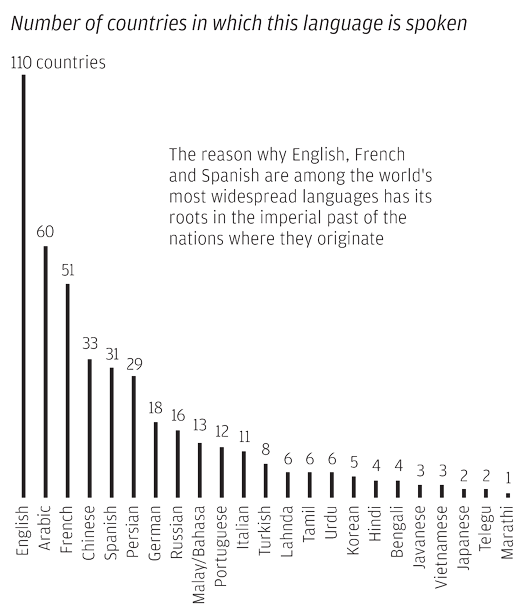
\includegraphics[width=100mm, keepaspectratio]{figures/countries_languages.png}
\caption{Országok száma, melyekben az adott nyelvet beszélik.}
\end{figure}

% https://www.visualcapitalist.com/wp-content/uploads/2018/05/world-of-languages.html

Számos nyelvet beszélnek világszerte az angol mellett, sokak számára viszont az angol nem az anyanyelvük, estleg egyáltalán nem beszélik azt. Beszédfelismerés során tehát szükséges egyéb hivatalos nyelveket is vizsgálni és kutatni.

Oroszország politikai és kulturális befolyása a világ ügyeibe vitathatatlan, így az orosz nyelv is fontos szerepet tölt be a nemzetközi porondon. Az 1.1-es ábrán látható, hogy elterejedt nyelvnek számít több országban is. Az end-to-end technológia és a neurális hálók által nyújtott lehetőségek megkönnyítik a nyelvek közti átállást, így egy angoltól eltérő nyelv vizsgálata és kutatása gördülékenyen megvalósítható egy angol nyelvű példa alapján.

\section{Megoldások}

A beszédfelismerő rendszereket pontosságuk alapján tudjuk rangsorolni. Egy nemzetközileg elismert pontossági mérőszám a WER (Word Error Rate). Ezt a pontosságot szokás szerint egy publikusan elérhető, angol nyelvű hangoskönyv felolvasásokat tartalamzó adatbázison, a LibriSpeech-en\footnote{LibriSpeech oldala: \url{http://www.openslr.org/12/}} mérik.

Különböző, alacsony hibaarányú modellek léteznek, de ez egyik lekiemelkedőbb közülök az Nvidia QuartzNet\footnote{Az Nvidia ismertető oldala: \url{https://developer.nvidia.com/blog/develop-smaller-speech-recognition-models-with-nvidias-nemo-framework/}} modelje, mely alacsonyszámú paraméterek mellett képes igen nagy preciziót fenntartani. Míg a QuartzNet bonyolultsága, paramétereinek a száma csupán töredéke a legtöbb SOTA modellének, a WER száma megközelíti azokét (1.1-es táblázat).

A modellekben elterjedt a konvolúciós- (CNN) és rekurrens neurális rétegek  (RNN) használata.

\begin{table}[ht]
	\footnotesize
	\centering
	\begin{tabular}{ p{2cm} p{2.5cm} p{2.5cm} p{1.5cm} p{1.5cm} p{1.5cm} }
		\toprule
		\textbf{Model} & \textbf{Aug} & \textbf{LM} & \textbf{clean WER(\%)} & \textbf{other WER(\%)} & \textbf{Million Parameters} \\
		\midrule
		wav2letter++ & Speed Perturb & ConvLM & 3.26 & 10.47 & 208 \\
		\hline
		LAS & SpecAugment & RNN & 2.5 & 5.8 & 360 \\
		\hline
		Time-Depth Separable Convolutions & Dropout, Label Smoothing & N/A (greedy) & 5.36 & 15.64 & 37 \\
		&  & 4-gram & 4.21 & 11.87 &  \\
		&  & ConvLM & 3.28 & 9.84 &  \\
		\hline
		Multi-Stream Self-Attention & Speed Perturb & 4-gram & 2.93 & 8.32 & 23  \\
		&  & 4-LSTM & 2.20 & 5.82 &  \\
		\hline
		QuartzNet-15x5 & Spec Cutout, Speed Perturb & N/A (greedy) & 3.90 & 11.28 & 19 \\
		&  & 6-gram & 2.96 & 8.07 &  \\
		&  & Transformer-XL & 2.69 & 7.25 &  \\
		\bottomrule
	\end{tabular}
	\caption{Angol nyelven tanult SOTA beszédfelismerő modellek és paramétereik.}
\end{table}

\section{Összefoglaló}

Megoldásomban az Nvidia QuartzNet alapján indultam el, annak alacsony paraméterszámát figyelembe véve. Egy Pytorch alapú toolkit-et, az Nvidia NeMo-t (Neural Modules) használva kísérleteztem QuartzNet kombinációkkal.

Főként az ingyenesen hozzáférhető Mozilla Common Voice adatbázist haszálva tanítottam orosz nyelvre a legsikeresebbnek ítélt, 15x5 architektúrájú modellt. A modellt nem véletlenszerűen beállított súlyokkal, hanem transfer learning-et alkalmazva, egy előre tanított angol modellbeli súlyokkal inicilaizáltam.

Az eredmény finomítása végett próbálkoztam több tanítóadat beiktatásával, mellyel a validációs adathalmaz WER értéke csökkent, így javult. Sajnos a több tanítóadat lényeges megnövelte a tanítás idejét így erőforrások szűkében csökkentette a kísérletezésre jutó időt, ezért ezt a módszert csak kis mértékben alkalmaztam.

\section{Diplomaterv felépítése}

A feladatkiírás elemzése fejezetben a sarkalatos pontok kerülnek részletezésre, kifejtésre. Ezen pontok kidolgozásának lehetőségei, esetleges nehézségei kerülnek említésre a felsorakoztatva a tervezés előtt felmerült, megvalósított és elvetett ötleteket.

Az előzmények és irodalomkutatás rész az eddigi megoldásokat részletezi és veti össze, röviden értékelve azok sikerességét. A levonható következtetések fényében felsorakoztat néhány későbbi tervezésbeli döntést.

A tervezés fejeztet magába foglalja az előzetes döntéseket, a lehetséges kísérletek várható eredményét, a döntési lehetőségeket értékelve és az azok mögötti ötleteket, esetleges alternatívákkal kiegészítve. A végső soron válaszott megoldások alátámasztása és indoklása is megjelenik a részben.

Az összefoglaló tartalmazza az elért eredmények bemutatását, azok értékelését és a végső következtetések levonását.